\documentclass{ximera}
%\usepackage{todonotes}

\usepackage{tkz-euclide}
\usetikzlibrary{backgrounds} %% for boxes around graphs
\usetikzlibrary{shapes,positioning}  %% Clouds and stars
\usetkzobj{all}
\usepackage[makeroom]{cancel} %% for strike outs
%\usepackage{mathtools} %% for pretty underbrace % Breaks Ximera
\usepackage{multicol}


\newcommand{\RR}{\mathbb R}
\renewcommand{\d}{\,d}
\newcommand{\dd}[2][]{\frac{d #1}{d #2}}
\renewcommand{\l}{\ell}
\newcommand{\ddx}{\frac{d}{dx}}
\newcommand{\zeroOverZero}{$\boldsymbol{\tfrac{0}{0}}$}
\newcommand{\numOverZero}{$\boldsymbol{\tfrac{\#}{0}}$}
\newcommand{\dfn}{\textbf}
\newcommand{\eval}[1]{\bigg[ #1 \bigg]}
\renewcommand{\epsilon}{\varepsilon}
\renewcommand{\iff}{\Leftrightarrow}

\DeclareMathOperator{\arccot}{arccot}
\DeclareMathOperator{\arcsec}{arcsec}
\DeclareMathOperator{\arccsc}{arccsc}


\colorlet{textColor}{black} 
\colorlet{background}{white}
\colorlet{penColor}{blue!50!black} % Color of a curve in a plot
\colorlet{penColor2}{red!50!black}% Color of a curve in a plot
\colorlet{penColor3}{red!50!blue} % Color of a curve in a plot
\colorlet{penColor4}{green!50!black} % Color of a curve in a plot
\colorlet{penColor5}{orange!80!black} % Color of a curve in a plot
                                      \colorlet{fill1}{blue!50!black!20} % Color of fill in a plot
\colorlet{fill2}{blue!10} % Color of fill in a plot
\colorlet{fillp}{fill1} % Color of positive area
\colorlet{filln}{red!50!black!20} % Color of negative area
\colorlet{gridColor}{gray!50} % Color of grid in a plot

\pgfmathdeclarefunction{gauss}{2}{% gives gaussian
  \pgfmathparse{1/(#2*sqrt(2*pi))*exp(-((x-#1)^2)/(2*#2^2))}%
}



\newcommand{\fullwidth}{}
\newcommand{\normalwidth}{}



%% makes a snazzy t-chart for evaluating functions
\newenvironment{tchart}{\rowcolors{2}{}{background!90!textColor}\array}{\endarray}

%%This is to help with formatting on future title pages.
\newenvironment{sectionOutcomes}{}{} 

\author{Emma Smith Zbarsky}
\license{Creative Commons Attribution 3.0 Unported}
\acknowledgement{https://quadbase.org/questions/q14498v1}
\begin{document}

\begin{exercise}

A pine tree 96 feet tall casts a shadow on the ground. How is the length
of the shadow changing when the acute angle between the sun and the
ground is $\pi/6$ radians? Assume the angle between the sun and the
ground changes at a constant rate of $\pi/12$ radians per hour.



\begin{image}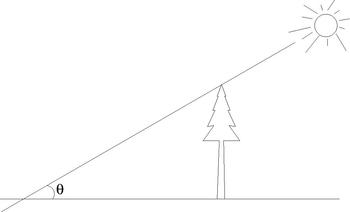
\includegraphics{relatedrates-tree.jpg}\end{image}


\begin{hint}
This is a related rates problem. You need to identify and label the
variables and find a relation between them. Then differentiate the
relation and use your known values and rates to compute the desired
rate.
\end{hint}


\begin{hint}
\begin{image}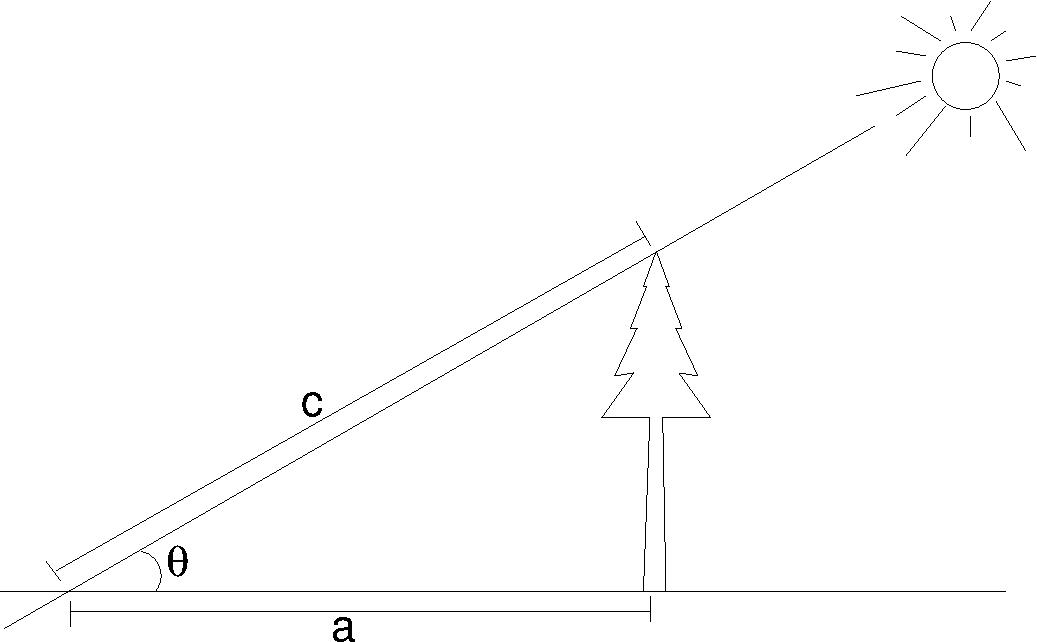
\includegraphics{rr-tree-labeled.jpg}\end{image}



Variables

\begin{itemize}
\item
  $a$ the length of the shadow in feet
\item
  $c$ the length of the hypotenuse of the shadow/tree triangle in feet
\item
  $\theta$ the acute angle between the ground and the sun in radians
\end{itemize}

Relation

\begin{itemize}
\item
  $a^2+96^2 = c^2$ (not useful - no $\theta$)
\item
  $\tan(\theta) = \frac{96}{a}$ (useful! has both $\theta$ and $a$)
\end{itemize}

Differentiating the useful relation, we have

\begin{itemize}
\itemsep1pt\parskip0pt\parsep0pt
\item
  $\sec^2(\theta)\frac{d\theta}{dt} = -\frac{96}{a^2}\frac{da}{dt}$
\end{itemize}

Knowns

\begin{itemize}
\item
  Tree is 96 feet tall
\item
  $\frac{d\theta}{dt} = \frac{\pi}{12}$ radians/hour
\item
  $\theta = \frac{\pi}{6}$ radians at the time of interest
\end{itemize}

Therefore, $\tan(\pi/6) = \frac{96}{a}$ and $a = 96\sqrt{3}$ feet

Plugging in our known (and computed) values for $a$, $\theta$ and
$\frac{d\theta}{dt}$ we have \begin{align*}
\sec^2(\theta)\frac{d\theta}{dt} &= -\frac{96}{a^2}\frac{da}{dt}\\
\sec^2(\pi/6)\left(\frac{\pi}{12}\right) &= -\frac{96}{(96\sqrt{3})^2}\frac{da}{dt} \\
\left(\frac{2}{\sqrt{3}}\right)^2\frac{\pi}{12} &= -\frac{1}{96\cdot 3}\frac{da}{dt} \\
\frac{da}{dt} &= -\frac{\pi}{9}\left(96\cdot 3\right)  \\
&= -32\pi
\end{align*} So the length of the shadow is changing at $-32\pi$ feet
per hour when $\theta = \pi/6$.
\end{hint}


\begin{multipleChoice}
\choice{$-\frac{32}{9}\pi$ feet per hour}
\choice{$96\pi$ feet per hour}
\choice[correct]{$-32\pi$ feet per hour}
\choice{$\frac{32}{9}\pi$ feet per hour}
\choice{$32\pi$ feet per hour}
\choice{$-96\pi$ feet per hour}
\end{multipleChoice}

\end{exercise}
\end{document}
